\section{Mathematische Modelle \skript{27}}
\subsection{Deskriptive Modelle und Optimierungsmodelle \skript{27}}
  \begin{tabular}{|p{3.7cm}|p{7cm}|p{7cm}|}
    \hline
    & \textbf{Deskriptive Modelle}
    & \textbf{Optimierungsmodelle} \\
    \hline
    \hline
    Antworten auf\ldots
      & ``What if?''
      & ``What's best?'' \\
    \hline
    Mengen ($I$)
      & \multicolumn{2}{l|}{Typen von Objekten (z.B. Städte $I = {1,2,\ldots,n}$)} \\
    \hline
    Parameter ($p_i$)
      & \multicolumn{2}{p{14cm}|}{Vorgebene Grössen des Modells (z.B. aktueller Fahrzeugbestand in Filiale $i$, Distanz zwischen Filiale $i$ und $j$)} \\
    \hline
    Variablen ($x_{ij}$)
      & \multicolumn{2}{l|}{Veränderbare Modellgrösse (z.B. Anz. transferierte Fahrzeuge von Filiale $i$ nach $j$)} \\
    \hline
    Konsequenzen ($k_{i}, k_i^{out}$)
      & Output des deskriptiven Modells (z.B. gesamte Fahrdistanz), $k_0 = f_0(x,p)$ 
      & -\\
    \hline
    Restriktionen / Constraints ($k_{i}, k_i^{out}$)
      & - 
      & Bedingungen auf den Konsequenzen (meist Ungleichungen oder Gleichungen)\\
    \hline
    Zielfunktion $\min$ oder $\max$
      & - 
      & Zu maximierende oder minimierende Konsequenz\\
    \hline
  \end{tabular}


\subsection{Allgemeines Optimierungsproblem \skript{31}}
  In Form von Ungleichungen und Gleichungen werden mögliche Lösungsmengen (\em solution spaces \em) definiert. Dort soll eine Zielfunktion $f$ optimiert (maximiert oder minimiert) werden. Die Fragestellung lautet: "`What's best?"' (preskriptive Modelle).
  
  \begin{center}
    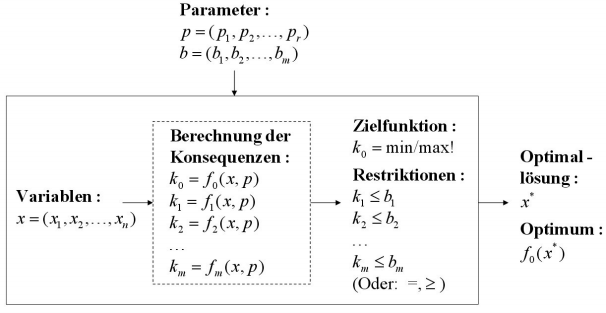
\includegraphics[width=10cm]{./Content/OptMathModels/OptimiziationModel}
  \end{center}
  
  \todo{Problemformulierung, Zulässigkeit, Beschränktheit, Abgeschlossenheit, Restriction, Unterscheidung Lokales-Globales Optimum, Eigenschaften von convexen und konkaven Funktionen}

\subsection{Konvexe Optimierung \skript{40}}
  Jedes lokale Optimierung entspricht einem globalen Optimum!
  
  Konvexe Menge:\\
  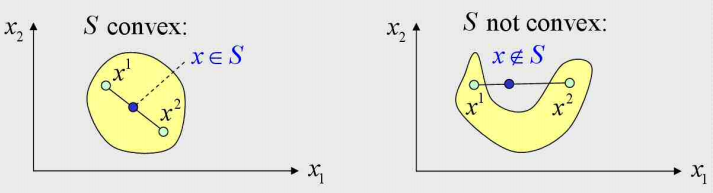
\includegraphics[width=8cm]{./Content/OptMathModels/ConvexSet}

\subsection{Typen von Optimierungsmodellen und -methoden \skript{46}}

